Denne sektion er baseret på \textbf{REF TIL ESSENCE}.
Konfigurationstabellen, \cref{tab:konfigurationsTabel}, der er beskrevet i denne sektion er den første konfigurationstabel af systemet.
Grunden til dette er fordi metoden kun skal være en grundsten for videre arbejde.
Når man skal lave videre arbejde er det vigtigt at kigge på de findings der er beskrevet i en konfigurationstabel.
Denne del er dog ikke udfyldt på grund af der ikke er fundet nogle findings endnu, disse vil dog blive beskrevet senere i \textbf{REF TIL FINDINGS SEKTIONEN}.
Denne konfigurationstabel har mange ligheder med den der er beskrevet i \citet{misc:faellesrapp}.
Grunden til dette er fordi det er samme målgruppe der udvikles til, endvidere udvikles der til PsyLog platformen der blev udviklet i \citet{misc:faellesrapp}.

En konfigurationstabel er lavet fordi det er vigtigt at alle udviklere ser på projektet på samme måde, så alle ved lige præcis hvad for et type projekt der arbejdes på, samt hvorfor lige præcis dette projekt udvikles.
Ydermere, giver konfigurationstabellen også et overblik over hvilket komponenter der kan bruges til at udvikle projektet, samt også hvilket begrænsninger der muligvis er i projektet.
Endvidere, beskriver konfigurationstabellen også en måde at evaluere projektet på, så alle ved præcis hvordan de skal evaluere vigtigheden af de forskellige opgaver.

Til at sørge for at alle udviklere har det samme vision for projektet er der lavet både en metafor, ikon og proposition.
Metaforen for system er en objektiv søvn dagbog, dette er valgt fordi det er sensorer der samler data og vedhjælp af disse lave en historie omkring hvordan ens søvn har været.
Ikonet for vores produkt er \textit{Sleep Cycle} \citep{misc:sleepCycle}, hvilket er en alarm applikation som vækker en når man er i den lette søvn periode.
Grunden til at dette er vores ikon er fordi det kun bruger de sensorer der er indbygget i ens telefon, og ud fra dem kan finde ud af hvor let man sover.

\winde{Tilføj manglende REFS}
\begin{figure}[h]
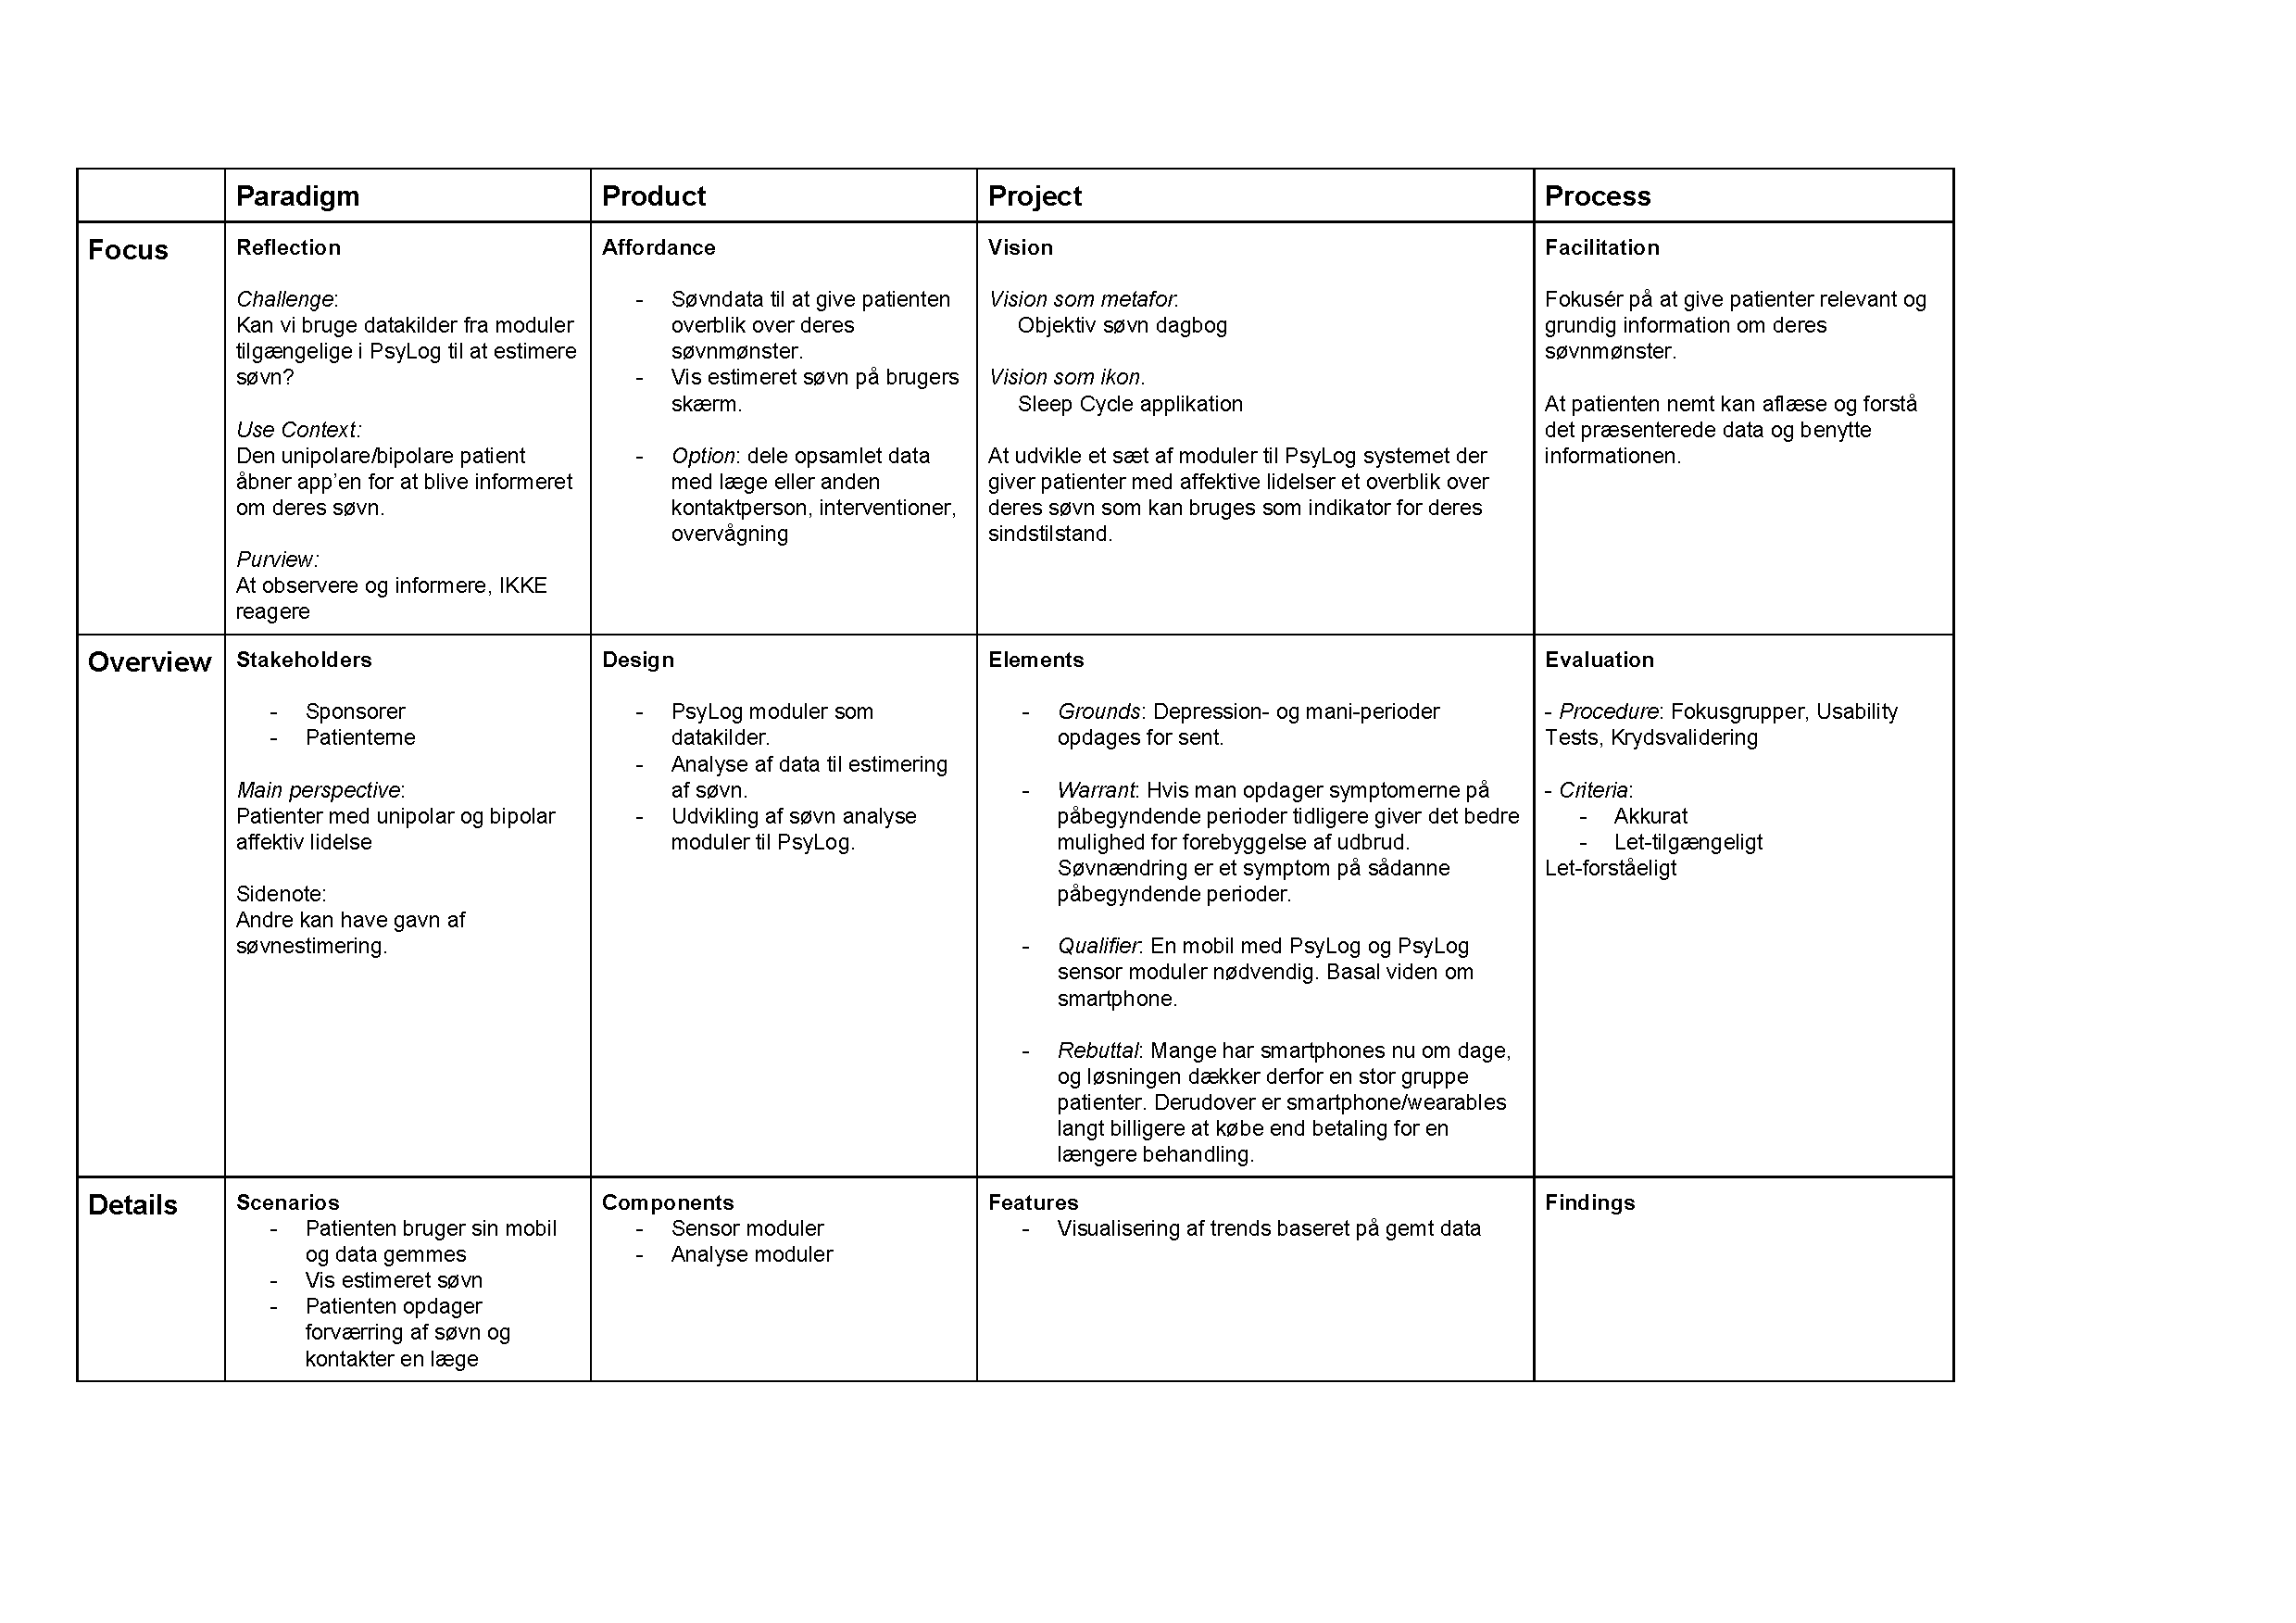
\includegraphics[scale = 0.45,trim = 1cm 3cm 6cm 2cm, clip]{konfigurationstabel}
\caption{Konfigurations tabellen for systemet.}
\label{tab:konfigurationsTabel}
\end{figure}